\documentclass[pdf]{beamer}
%\documentclass[pdf,handout]{beamer}
\mode<presentation>{\usetheme[secheader]{Boadilla}}
\usepackage{mystyle}
\includecomment{versiona}
\usepackage{xeCJK}
\usepackage{subfig}
\usepackage{soul}

%\setbeameroption{hide notes}
\newcommand{\red}[1]{{\color[rgb]{0.6,0,0}#1}}
\setCJKmainfont[AutoFakeBold=true]{Hiragino Mincho Pro} %my Mac
%\setCJKmainfont{MS PGothic} %AJP windows

\makeatletter
\newenvironment<>{proofs}[1][\proofname]{\par\def\insertproofname{#1\@addpunct{.}}\usebeamertemplate{proof begin}#2}
{\usebeamertemplate{proof end}}
\makeatother

\makeatletter
\def\th@mystyle{%
\normalfont % body font
\setbeamercolor{block title example}{bg=orange,fg=white}
\setbeamercolor{block body example}{bg=orange!20,fg=black}
\def\inserttheoremblockenv{exampleblock}
}
\makeatother

\newtheorem{question}{Question}
\newtheorem*{theorem*}{Theorem}
\theoremstyle{remark}
\newtheorem*{remark*}{Remark}

\renewcommand{\implies}{\Rightarrow}

\title{New Formula for Convolution of  Neural Networks}
\subtitle{joint with 小林俊行}
\author{レオンチエフ・アレックス、東大数理}

\begin{document}
\begin{frame}\titlepage\end{frame}
\begin{frame}
	Recall the content of the previous talk:
	\pause
	the following holds:
	\begin{equation}
		\begin{array}{l}
			  \int_{- 1}^1 \int_{- 1}^1 | s - t |^{2 \nu} (1 - s^2)^{\lambda -
				    \frac{1}{2}} (1 - t^2)^{\mu - \frac{1}{2}} C_l^{\lambda} (s) C_m^{\mu} (t) d
				      s d t\\
				        = \frac{(- \nu)_{\frac{l + m}{2}} (- 1)^{\frac{l - m}{2}} \pi^{\frac{1}{2}}
					  (2 \lambda)_l (2 \mu)_m \Gamma \left( \lambda + \frac{1}{2} \right) \Gamma
					    \left( \mu + \frac{1}{2} \right) \Gamma \left( \nu + \frac{1}{2} \right)
					      \Gamma (\lambda + \mu + 2 \nu + 1)}{l!m! \Gamma \left( \lambda + \nu +
						        \frac{l - m}{2} + 1 \right) \Gamma \left( \mu + \nu - \frac{l - m}{2} + 1
							  \right) \Gamma \left( \lambda + \mu + \nu + \frac{l + m}{2} + 1 \right)}
						    \end{array}
		\label{eqn:1}
	\end{equation}
	\pause From here, we easily derive two equivalent formulations:
	\begin{equation}
		\myabs{s-t}^{2 \nu} = \sum_{\ell, m = 0 \mid l + m : \mbox{even}}^{\infty}
		a_{\lambda, \mu, \nu}^{\ell, m} C_{\ell}^{\lambda} (s) C_m^{\mu} (t),
		\label{eqn:4}
	\end{equation}
	{\scriptsize 
	\begin{equation*}
 	a^{\ell,m}_{\lambda,\mu,\nu}=
	\frac{2^{- 2 \nu} (\lambda + \ell) (\mu + m) \Gamma (\lambda + \mu + 2 \nu +
1) \Gamma (\lambda) \Gamma (\mu) \Gamma (2 \nu + 1)}{\Gamma \left( \lambda +
	\nu + \frac{\ell - m}{2} + 1 \right) \Gamma \left( \mu + \nu - \frac{\ell -
	m}{2} + 1 \right) \Gamma \left( \lambda + \mu + \nu + \frac{\ell + m}{2} + 1
	\right) \Gamma \left( \nu + 1 - \frac{\ell + m}{2} \right)}
	,
	\end{equation*}
}
	\pause
	and
	\begin{equation}
		\begin{array}{c}
		\begin{array}{ccl}
			\int_{-\infty}^\infty\myabs{w}^{2 \nu} &\int_{-\infty}^\infty c_m^{\mu} (s - w) \;c^{\lambda}_l (s) {ds}{dw} &= \ldots,\\
			\mathcal{M} &\left( c_m^\mu \ast c_\ell^\lambda  \right)&=\dots
		\end{array}
		      \end{array}
		\label{eqn:2}
	\end{equation}
\end{frame}
\begin{frame}
	Here
	\begin{equation*}
		c^{\lambda}_\ell (s) =\left\{\begin{array}{ll}
			      (1 - s^2)^{\lambda - \frac{1}{2}} C^{\lambda}_\ell (s),&-1\le s\le1,\\
			      0,&\mbox{otherwise.}
		\end{array}\right.
		\label{eqn:3}
	\end{equation*}
	and
	\begin{equation*}
		\left\{ \mathcal{M}(f) \right\}(s)=\int_0^\infty x^{s-1}f(x)dx	
	\end{equation*} is the Mellin transform.
	\pause
	Taking the inverse Mellin transform\begin{equation*}
		\left\{ \mathcal{M}^{-1}(\varphi) \right\}(x)=\frac{1}{2\pi i}\int_{c-i\infty}^{c+i\infty}x^{-s}\varphi(s)ds
	\end{equation*}of \eqref{eqn:3}, we get the closed formula for convolution of $c_{\ell}^\lambda$.
\end{frame}
\begin{frame}{Machine Learning is Function Approximation}
	\begin{figure}[h]
		\centering
		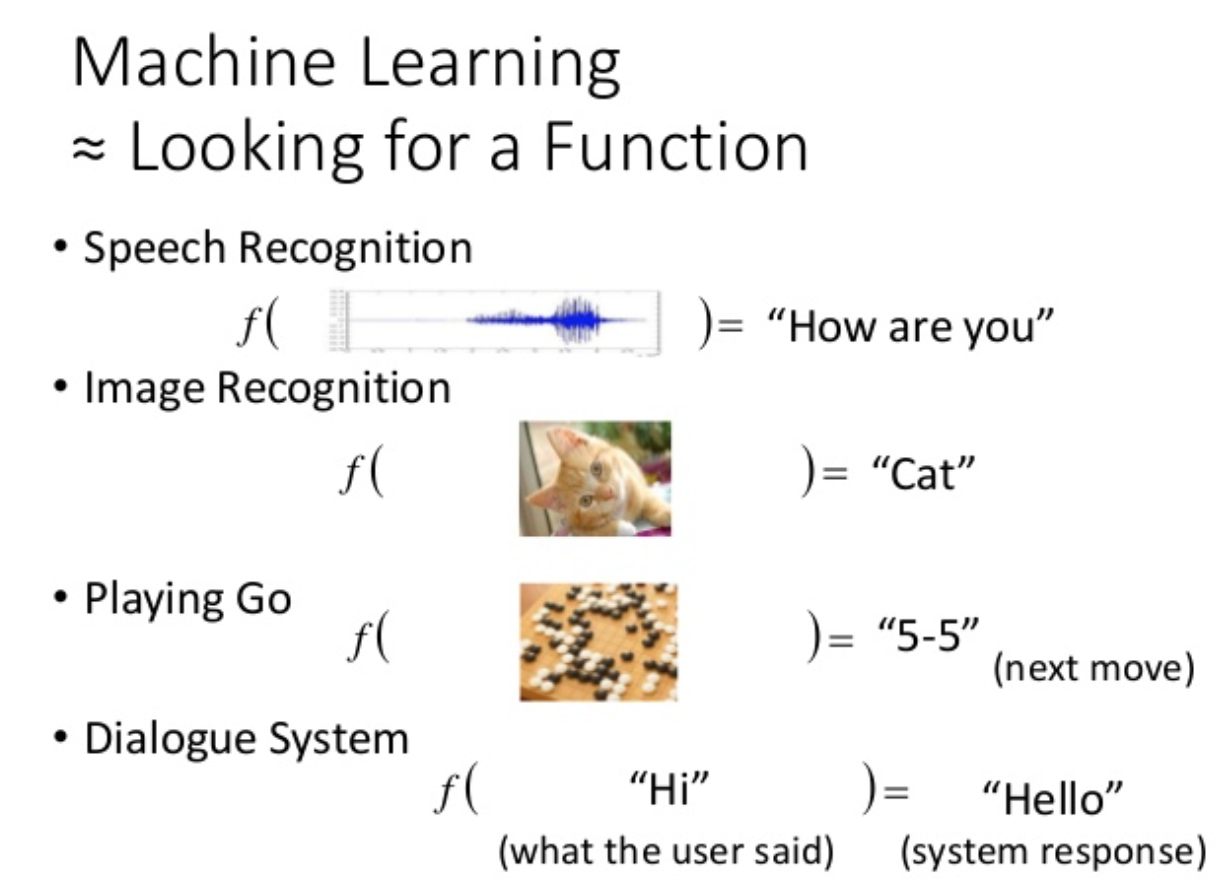
\includegraphics[scale=0.49]{mlisfa}
		%\note{tesime}
	\end{figure}
\end{frame}
\begin{frame}
	\begin{figure}[h]
		\centering
		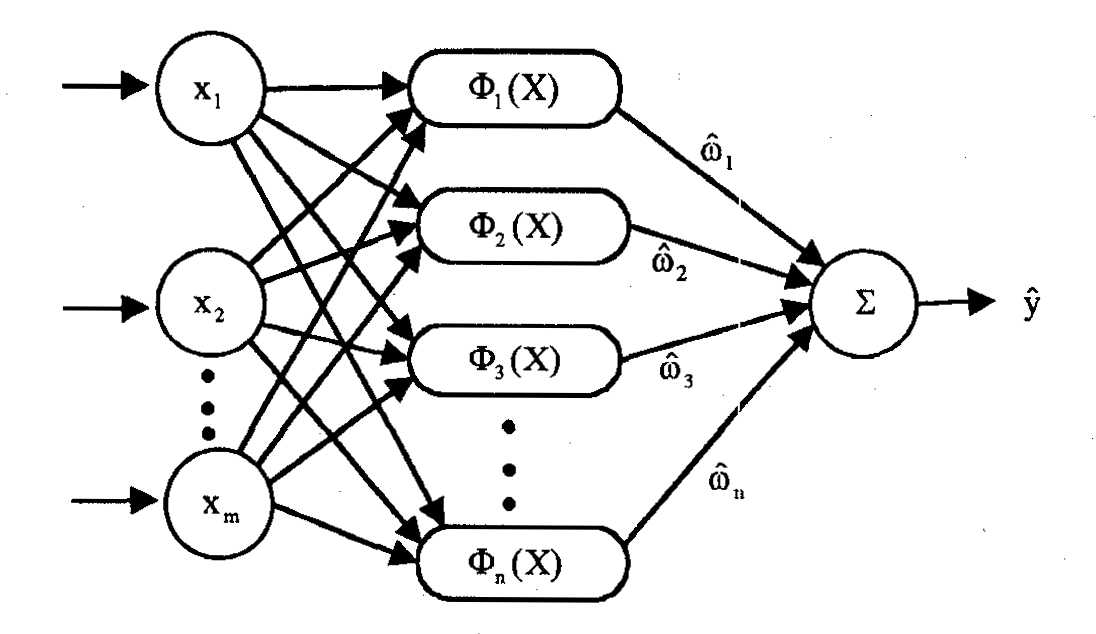
\includegraphics[scale=0.3]{onn}
		\caption{Orthogonal Neural Network (taken from \cite{yang1996orthogonal})}
		\label{fig:onn}
		%\note{tesime}
	\end{figure}
	\begin{block}{Idea}
		Approximate signal $y(x)$ using orthogonal functions:\begin{equation*}
			y(x)\approx \hat{y}(x):=\sum_{i=1}^N \hat{\omega}_i  \Phi_i(x)
		\end{equation*}
	\end{block}
	This connects neural networks with functional analysis!
\end{frame}
\begin{frame}{Advantages}
	\begin{itemize}
		\item Architecture is simple\only<2>{ (cf. deep learning)};
		\item<-1> Parameters are few;
		\item<-1> Can choose particular OFs to suit the particular problem domain (e.g. Hermite functions for medical imaging);
		\item<-1> Error estimation is readily available ($\implies$ can estimate convergence speed);
		\item<-1> Many strategies for the training of coefficients; 
		\item<-1> For some OFs we can use recurrence relations to speed up the computation (e.g. Lagrange, Hermite functions/polynomials)
	\end{itemize}
\only<1>{
\begin{figure}
  \centering
  \vspace{-0.6cm}
  \subfloat{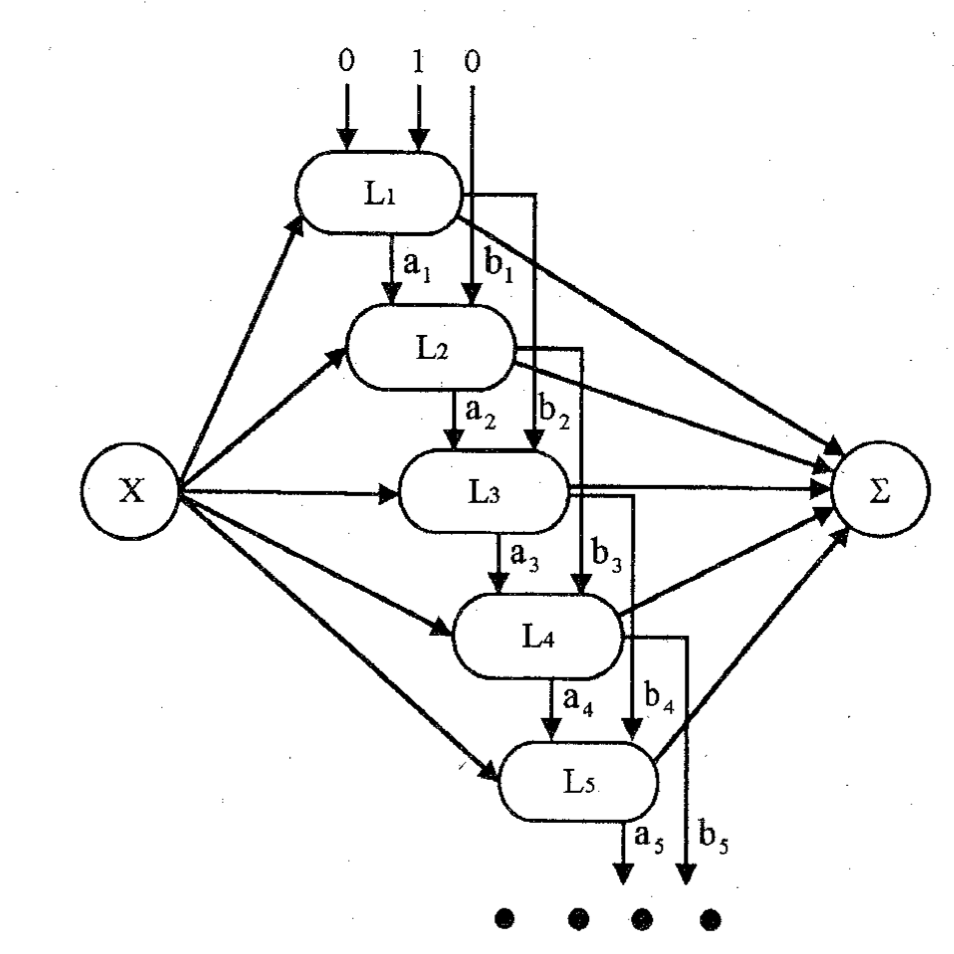
\includegraphics[scale=0.2]{onn2}}\qquad
  \subfloat{\raisebox{0.5cm}{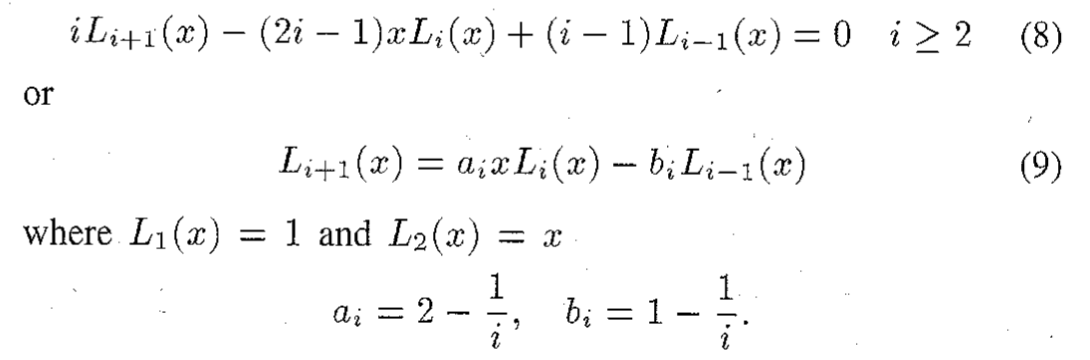
\includegraphics[scale=0.4]{onn3}}}
\caption{(taken from \cite{yang1996orthogonal})}
\end{figure}
}
\only<2>{
	\vspace{-4cm}
	\begin{theorem*}[Universal approximation theorem {\cite{cybenko1989approximation,hornik1989multilayer}}]
		Let $\varphi$ be nonconstant, bounded and monotonically-increasing continuous function.
		Then,  $\forall\varepsilon>0,\exists N,\forall f\in C([0,1]^m)\exists v_i,b_i\in\R,w_i\in\R^m$ such that
		for $F(x):=\sum_{i=1}^Nv_i\varphi(w_i^Tx+b_i)$ we have $\mynorm{f-F}_{\infty}<\varepsilon$.
\end{theorem*}
\begin{remark*}
	Informally, this theorem tells that any reasonable function can be approximated
	with network having only \underline{one hidden layer}, but being wide enough.

	In some sense, this is an \underline{anti deep-learning} result.
\end{remark*}
}
\end{frame}
%%\begin{frame}{Why Hermite Networks?}
%%	\begin{equation*}
%%		\begin{array}[]{c}
%%			h_n(t)=\frac{H_n(t)e^{-t^2/2}}{\sqrt{2^nn!\sqrt{\pi}}}\mbox{ (Hermite {\it functions})};\\
%%		H_n(t)=(-1)^n e^{t^2}\frac{d^n}{dt^n}e^{-t^2}\mbox{ (Hermite {\it polynomials})}.
%%		\end{array}
%%	\end{equation*}
%%	
%%	\begin{itemize}
%%		\item Low order Hermite functions resemble some important signals in biomedical engineering \cite{mackenzie2003hermite};
%%		\item Recursive formula $H_{n+1}(t)=2tH_n(t)-2nH_{n-1}(t)$ (see above);
%%		\item Can be implemented in hardware \cite{osowski1992neural,cochocki1993neural,chesnokov1999new};
%%	\end{itemize}
%%	Besides, good analytic properties:
%%	\begin{itemize}
%%		\item Invariant under Fourier transform: $\mathcal{F}(h_n)=\left( -i \right)^n\sqrt{2\pi}h_n$ $\left( \implies
%%			\mathcal{F}\left( \hat{y} \right)=\sum_{j=1}^N \hat{\omega}_j (-i)^j \sqrt{2\pi}h_j \right)$;
%%			
%%		\item $h_0$ is the Gaussian filter\vspace{-0.5cm}\begin{equation*}
%%				\implies e^{-t^2/2}\ast y\approx e^{-t^2/2} \ast \hat{y} =\sum_{i=1}^N \hat{\omega}_i \left( h_i\ast h_0 \right)
%%			\end{equation*}
%%			\vspace{-0.5cm}
%%	\end{itemize}
%%\end{frame}
\begin{frame}{Why Convolution? (e.g. Hermitian Networks)}
	We often need to convolve two Hermite Neural Networks (e.g. to recover noised signal with Gaussian):
	\begin{equation*}
		y_1\ast y_2\approx \hat{y}_1\ast \hat{y}_2=\sum_{i,j=1}^N a^{(1)}_i a^{\left( 2 \right)}_j \left(h_i\ast h_j  \right)
	\end{equation*}
	
	It is good that we have an explicit formula:
	\begin{equation*}
		\left( h_i\ast h_j \right)(t)=\left\{\begin{array}[]{ll}
			\left( -1 \right)^{i+j}l_j^{i-j}\left( \frac{t^2}{2} \right),&t\ge0\\
			l_{j}^{i-j}\left( \frac{t^2}{2} \right),&t<0
		\end{array}\right.(j\le i).
	\end{equation*}
	
	\begin{itemize}
		\item There are fast algorithms to compute special functions/polynomials (e.g. recursive relations);
		\item Can do asymptotic analysis and error estimate very precise;
	\end{itemize}
\end{frame}
\begin{frame}
	And \eqref{eqn:3} gives us a closed formula for the convolution of
	\begin{equation*}
		c^{\lambda}_\ell (s) =\left\{\begin{array}{ll}
			      (1 - s^2)^{\lambda - \frac{1}{2}} C^{\lambda}_\ell (s),&-1\le s\le1,\\
			      0,&\mbox{otherwise.}
		\end{array}\right.
	\end{equation*}
	\pause
	Note that $\left\{ c^\lambda_\ell \right\}_{\ell=0}^\infty$ form an orthonormal basis of 
	\begin{equation*}
	L^2([-1,1],(1-x^2)^{\frac{1}{2}-\lambda}dx).
	\end{equation*}
	$\rightsquigarrow$ we can build on Orthogonal Neural Network based on them.
	\pause
	\begin{question}
		Which signals are suitable for approximation by $c^\lambda_{\ell}$? (cf. remark below)
	\end{question}
	\begin{remark*}
		Hermite Neural Networks
		are used in biomedical engineering, since
		Hermite functions bear some resemblance to the impulse response signals received from electrically stimulated organs \cite{mackenzie2003hermite}.
	\end{remark*}
\end{frame}
\begin{frame}{Mathematical formulation}
	Suppose $f\in 
	L^2([-1,1],(1-x^2)^{\frac{1}{2}-\lambda}dx)$. Expand it as\begin{equation*}
		\begin{array}{c}
			f(x)=\sum_{\ell=0}^\infty c_\ell \cdot c_\ell^\lambda(x)=\sum_{\ell=0}^\infty c_\ell \cdot(1-x^2)^{\lambda-\frac{1}{2}}C^\lambda_{\ell}(x),\\
			c_\ell=\frac{\ell!(\ell+\lambda)\Gamma(\lambda)^2}{\pi2^{1-2\lambda}\Gamma(\ell+2\lambda)}\int_{-1}^1 f(x)C^\lambda_\ell(x)dx.
		\end{array}
	\end{equation*}
	\begin{question}
		What conditions on $f$ correspond are sufficient for the \underline{fast decay} of $c_\ell$?
	\end{question}
\end{frame}
\begin{frame}{Model result}
	\begin{question}
		What conditions on $f$ correspond are sufficient for the \underline{fast decay} of $c_\ell$?
	\end{question}
	This is question is motivated by the following fact:
	\begin{theorem*}[{\cite[Thm. 2.2]{kashiwara1979k}}]
		Let $f$ be a function on a circle $\Sp^1$ and $f(x)=\sum_{\ell=0}^\infty c_\ell e^{i\ell x}$ be its Fourier series. Then,
		\begin{enumerate}
			\item $f\in\mathcal{A}$ if and only if $\exists C,\varepsilon>0\mid \myabs{c_\ell}<Ce^{-\varepsilon\ell}$;
			\item $f\in C^\infty$ if and only if $\forall m\in\N,\exists C_m>0$ such that $\myabs{c_\ell}<C_m(1+\ell)^m$;
			\item $f\in L^2$ if and only if $\sum_{\ell\ge0}\myabs{c_\ell}^2<\infty$;
			\item $f\in \mathcal{D}'$ if and only if $\exists m\in\N,C>0$ such that $\myabs{c_\ell}< C(1+\ell)^{m}$;
			\item $f\in \mathcal{B}$ if and only if for any $\varepsilon>0,\exists C_\varepsilon>0$ such that $\myabs{c_\ell}<C_\varepsilon e^{\varepsilon\ell}$.
		\end{enumerate}
	\end{theorem*}
\end{frame}
\begin{frame}{Possible approach}
	The reasonable starting point is to consider $\lambda=0,1$ as in this case Gegenbauer polynomials reduce to Chebyshev polynomials\begin{equation*}
		T_n(x)=\frac{n}{2}\lim_{q\to0}\frac{1}{q}C_n^q(x),\quad U_n(x)=C_n^1(x)
	\end{equation*}
	and these are related to sine and cosine series as\begin{equation*}
		T_n(\cos\theta)=\cos(n\theta),\quad U_n(\cos\theta)\cdot \sin\theta=\sin(n\theta).
	\end{equation*}
	Hence, we have\begin{equation*}
		t_\ell(\cos\theta):=\frac{\ell}{2}\lim_{q\to0}\frac{1}{q}c_\ell^q(x)=\frac{\ell}{2}\cdot\frac{\cos(\ell\theta)}{\sin\theta},\quad u_\ell(\cos\theta):=c^1_\ell(x)=\sin(\ell\theta)
	\end{equation*}
\end{frame}
\begin{frame}[allowframebreaks]
\frametitle{References}
\nocite{mackenzie2003hermite}
\nocite{yang1996orthogonal}
\bibliographystyle{apalike}
\bibliography{fmsp.bib}
\end{frame}
\end{document}
